\documentclass[10pt,aspectratio=43,mathserif]{beamer}		
%设置为 Beamer 文档类型,设置字体为 10pt,长宽比为16:9,数学字体为 serif 风格

%%%%-----导入宏包-----%%%%
\usepackage{seu}
\usepackage{xeCJK}
\usepackage{amsmath,amsfonts,amssymb,bm}
\usepackage{color}
\usepackage{graphicx,hyperref,url}	
%%%%%%%%%%%%%%%%%%


%%%%-----设置字体-----%%%%
%Windows和Mac OS下都可用
\setsansfont{Helvetica}

%\setsansfont{Times New Roman}

%仅Windows可用
%\setCJKmainfont{Hiragino Sans GB W3}

%仅Mac OS下可用
%\setCJKmainfont{Songti SC}




%设置 Beamer 主题
\beamertemplateballitem


\AtBeginSection[]
{
  \begin{frame}<beamer>
    \frametitle{\textbf{目录}}
    \textbf{\tableofcontents[currentsection]}
  \end{frame}
}


%%%%----首页信息设置----%%%%
\title[Sending out an SMS]{\fontsize{13pt}{18pt}\selectfont {Sending out an SMS: Characterizing the Security of the SMS Ecosystem with Public Gateways}}
\subtitle{\fontsize{9pt}{14pt}\selectfont \textbf{利用公共网关的SMS生态系统的安全性描述}}			
%%%%----标题设置


\author[R. Song]{
  Bradley Reaves, Nolen Scaife, Dave Tian, Logan Blue, \\
  Patrick Traynor and Kevin R.B. Butler \\\medskip
  {\small {\{reaves, scaife, daveti, bluel\}@ufl.edu}} \\
  {\small {\{traynor, butler\}@cise.ufl.edu}}}
%%%%----个人信息设置

\institute[FICS]{
  Florida Institute for Cybersecurity Research (FICS)\\
  University of Florida}
%%%%----机构信息

\date[\today]{
 \today}
%%%%----日期信息


\begin{document}

\begin{frame}
\titlepage
\end{frame}				%生成标题页



\section*{目录}

		\begin{frame}
		\frametitle{\textbf{目录}}
		\textbf{\tableofcontents}
		\end{frame}				%生成提纲页

\section{引言}

		\begin{frame}
			\frametitle{\textbf{引言}}
            \begin{block}{\textbf{研究背景}}
                \begin{itemize}
                    \item 短信息(SMS)成为现代通讯的重要组成部分
                    \item 很多组织或网站使用短信息作为身份验证的辅助通道
                    \item 现代短消息的发送,在抵达终端之前不接触蜂窝网络
                \end{itemize}
            \end{block}

            \begin{block}{\textbf{主要工作}}
                \begin{itemize}
                    \item 对SMS数据进行迄今为止最大的挖掘分析
                    \item 评估良性短消息服务的安全态势
                    \item 刻画通过SMS网关进行的恶意行为
                \end{itemize}
            \end{block}
        \end{frame}

\section[系统]{现代SMS生态系统}

		\begin{frame}
		  \frametitle{\textbf{短消息服务中心(SMSC)}}
            \begin{figure}[!t]
            \centering
            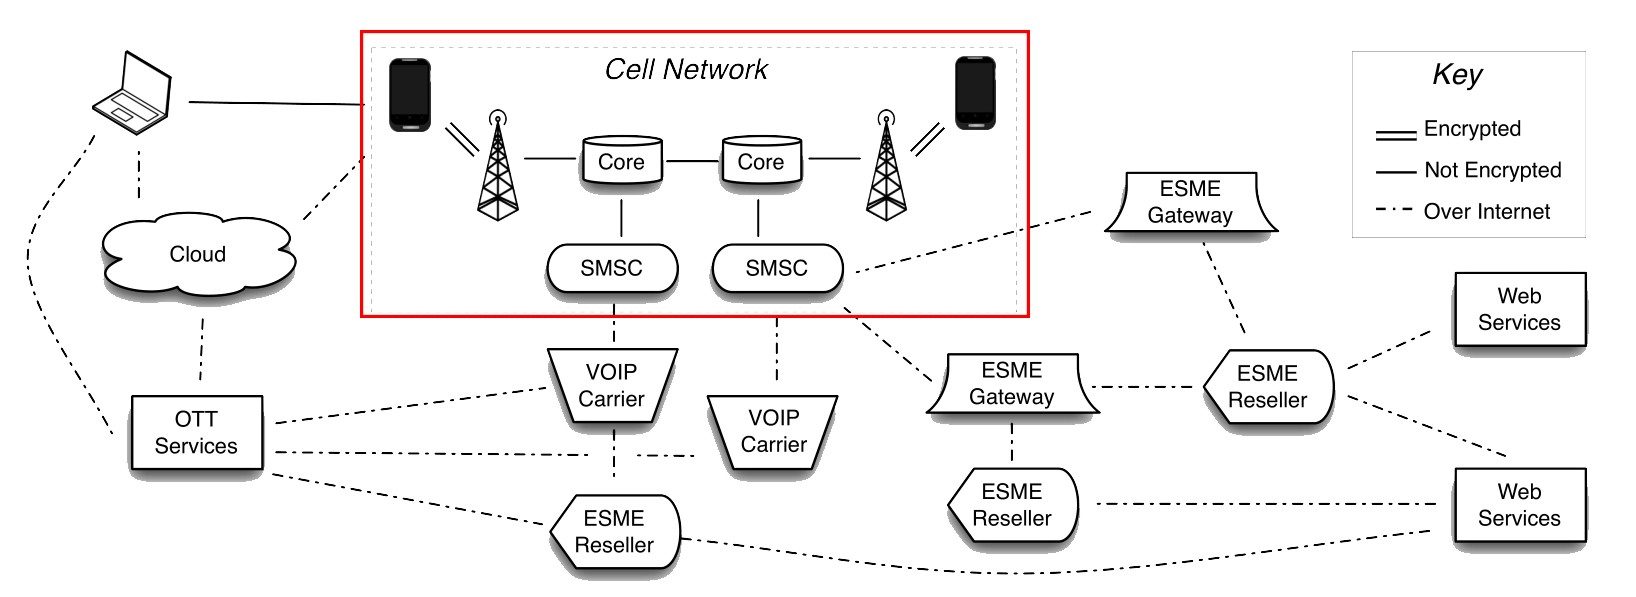
\includegraphics[width=4in]{figures/figure1.png}
            \caption{短消息服务中心}
            \label{figure1_SMSC}
            \end{figure}
            \textbf{短消息服务中心}通过运营商网络路由消息,是SMS系统的核心。\\
            SMSC接受文本消息,并将消息转发到蜂窝网络中的移动用户。
		\end{frame}

		\begin{frame}
		  \frametitle{\textbf{外部短消息实体(ESME)}}
            \begin{figure}[!t]
            \centering
            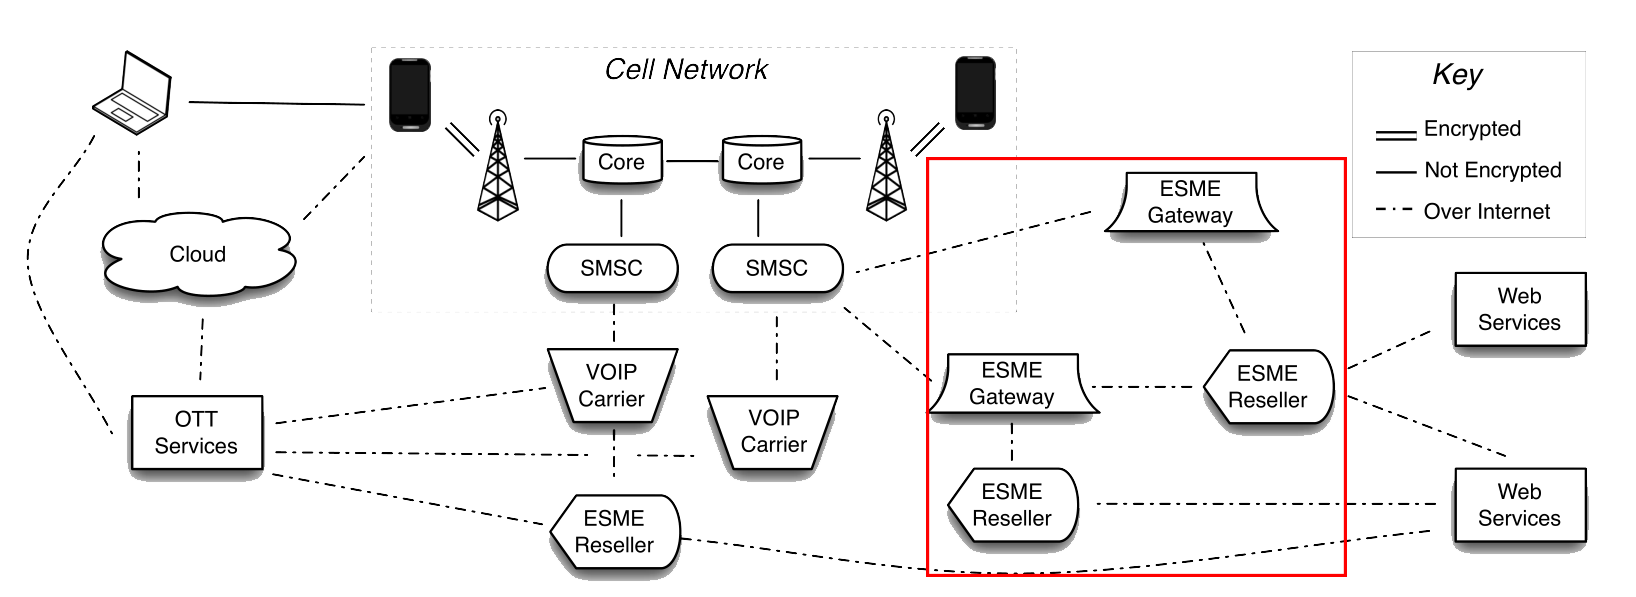
\includegraphics[width=4in]{figures/figure2.png}
            \caption{外部短消息实体}
            \label{figure2_ESME}
            \end{figure}
            \textbf{外部短消息实体}为外部组织提供针对运营商网络的短消息接入服务。\\
            ESME可以用于紧急通报、慈善捐款、或接受一次性验证码等功能。
		\end{frame}

        \begin{frame}
		  \frametitle{\textbf{OTT服务}}
			\begin{figure}[!t]
            \centering
            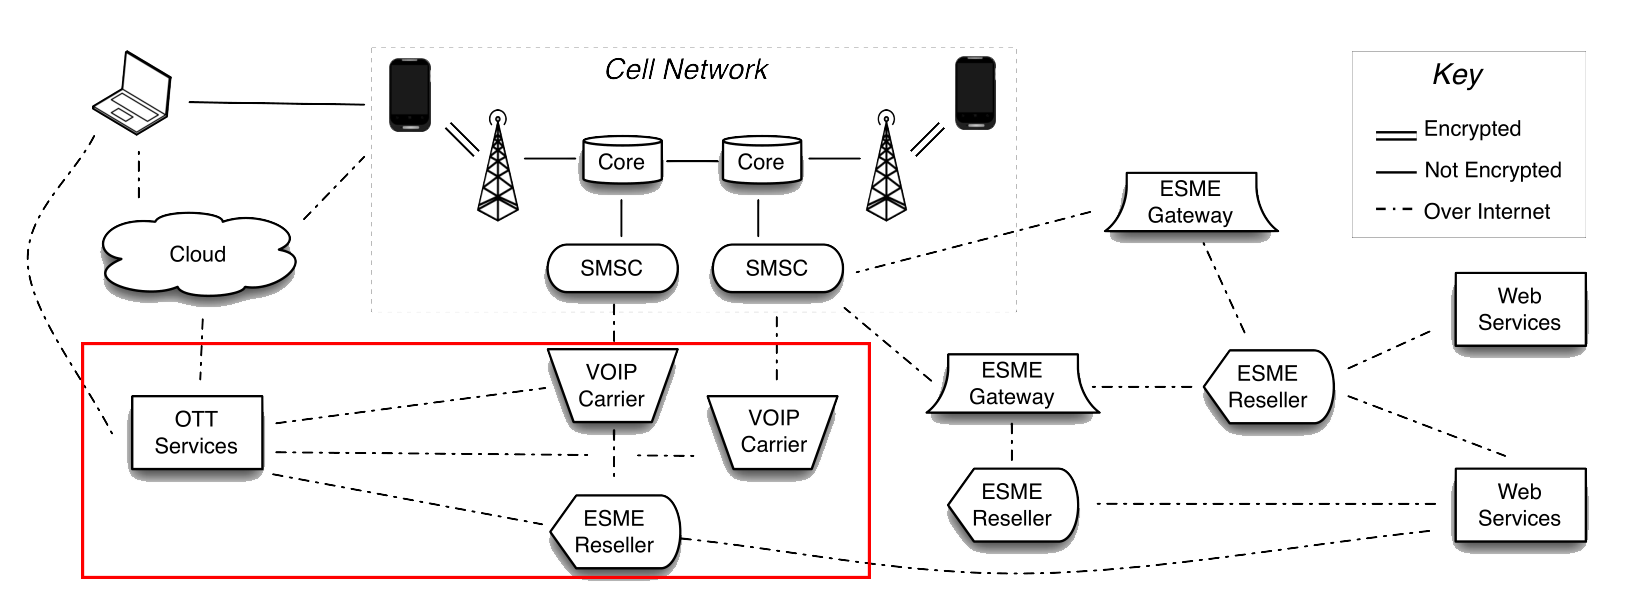
\includegraphics[width=4in]{figures/figure3.png}
            \caption{OTT服务}
            \label{figure3_OTT}
            \end{figure}
            \textbf{OTT服务}支持在数据网络上提供短信和语音等第三方服务。\\
            OTT可以使用云服务来存储和同步SMS到用户的其他设备。
		\end{frame}



\section[方法]{研究方法与数据集特征}


		\begin{frame}
		  \frametitle{\textbf{爬取公共短消息网关}}
            % ----------------分栏的结构开始---------------- %
            % 该结构中使用block分开两个内容区
            % 可根据需要进行图文混排?我还没试过,我想应该可以
            \begin{columns}
                \column{.5\textwidth}
                \footnotesize
                \begin{itemize}
                  \item 使用Scrapy框架爬取公共网关
                  \item 收集8个公共短信网关在14个月的数据
                  \item 共抓取386,327条数据
                \end{itemize}

                \column{.5\textwidth}
                \begin{table}
                \caption{公共网关及抓取的信息数}
                \label{table1:gateways}
                \centering
                \footnotesize
                \begin{tabular}{|c|c|}
                \hline
                \textbf{Site}           & \textbf{Messages}\\
                \hline
                receivesmsonline.net    &81313\\
                \hline
                receive-sms-online.info &69389\\
                \hline
                receive-sms-now.com     &63797\\
                \hline
                 hs3x.com               &55499\\
                \hline
                receivesmsonline.com    &44640\\
                \hline
                receivefreesms.com      &37485\\
                \hline
                receive-sms-online.com  &27094\\
                \hline
                 e-receivesms.com       &7107\\
                \hline
                \end{tabular}
                \end{table}
            \end{columns}

		\end{frame}

        \begin{frame}
		  \frametitle{\textbf{消息聚类分析}}
            \begin{block}{\textbf{基本思路}}
                \begin{itemize}
                    \item 使用编辑距离矩阵将类似的消息归于一张连通图中。
                    \item 使用固定值替换感兴趣的消息,如代码、email地址。
                    \item 查找归一化距离小于阈值的消息,并确定聚类边界。
                \end{itemize}
            \end{block}

            \begin{block}{\textbf{实现步骤}}
                \begin{enumerate}
                  \item 加载所有消息。
                  \item 用固定的字符串替换数字、电子邮件和URL以预处理消息。
                  \item 将预处理后的信息按字母排序。
                  \item 通过使用编辑距离阈值(0.9)来确定聚类边界。
                  \item 手动标记各个聚类,以确定服务提供者、消息类别等。
                \end{enumerate}
            \end{block}
		\end{frame}

        \begin{frame}
		  \frametitle{\textbf{消息分类结果}}
            \begin{itemize}
                \item \textbf{账户创建确认信息}:向来自服务提供者的用户提供了一个代码,该服务提供者需要在新帐户创建期间进行SMS验证。
                \item \textbf{活动确认信息}:向来自服务提供者的用户提供了请求授权进行活动的代码(例如,付款确认)。
                \item \textbf{一次性密码}:包含用户登录的代码的短信息。
                \item \textbf{用于绑定不同设备的一次性口令}:将消息发送给用户,以绑定一个新的电话号码或启用相应的移动应用程序。
                \item \textbf{重置密码口令}:包含密码重置密码的短信息。
                \item \textbf{其他}:其他未被指定为某种特定功能的消息。
            \end{itemize}
		\end{frame}

        \begin{frame}
		  \frametitle{\textbf{消息分类结果}}
            \begin{columns}
                \column{.5\textwidth}
                \footnotesize
                \begin{itemize}
                  \item 账户创建和移动设备绑定占比最大,占51.6\%
                  \item 一次性密码信息占7.6\%
                  \item 密码重置消息占1.3\%
                  \item 包含“测试”关键词的消息占0.8\%
                \end{itemize}

                \column{.5\textwidth}
                \begin{figure}[!t]
                    \centering
                    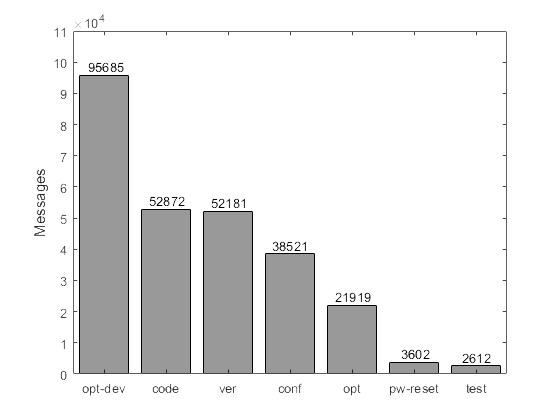
\includegraphics[width=1.1\textwidth]{figures/figure4.png}
                    \caption{消息的聚类}
                    \label{figure3_OTT}
                \end{figure}
            \end{columns}
		\end{frame}



\section[分析]{SMS使用情况分析}


		\begin{frame}
		  \frametitle{\textbf{使用SMS作为安全信道}}
		  \begin{block}{\textbf{PII和其他敏感信息}}
                \begin{itemize}
                    \item 财务信息
                    \item 用户名和密码
                    \item 重置密码口令
                    \item 其他个人识别信息(PII)
                    \item 敏感程序的SMS活动
                \end{itemize}
            \end{block}
		\end{frame}

        \begin{frame}
		  \frametitle{\textbf{使用SMS作为安全信道}}
            \begin{block}{\textbf{SMS编码熵}}
                使用 $\chi$方检验测试每组编码的熵。$\chi$方检验是一个零假设的显著性检验,用于测试SMS服务的编码是否是从低位到高位均匀分布的。若p值小于0.01,则表明观测值和理想均匀分布之间存在统计学上的显著差异。
                检验结果表明,65\%的SMS服务的编码熵较低,容易被预测和攻击。
            \end{block}
            \begin{columns}

                \column{.26\textwidth}
                \begin{figure}
                    \centering
                    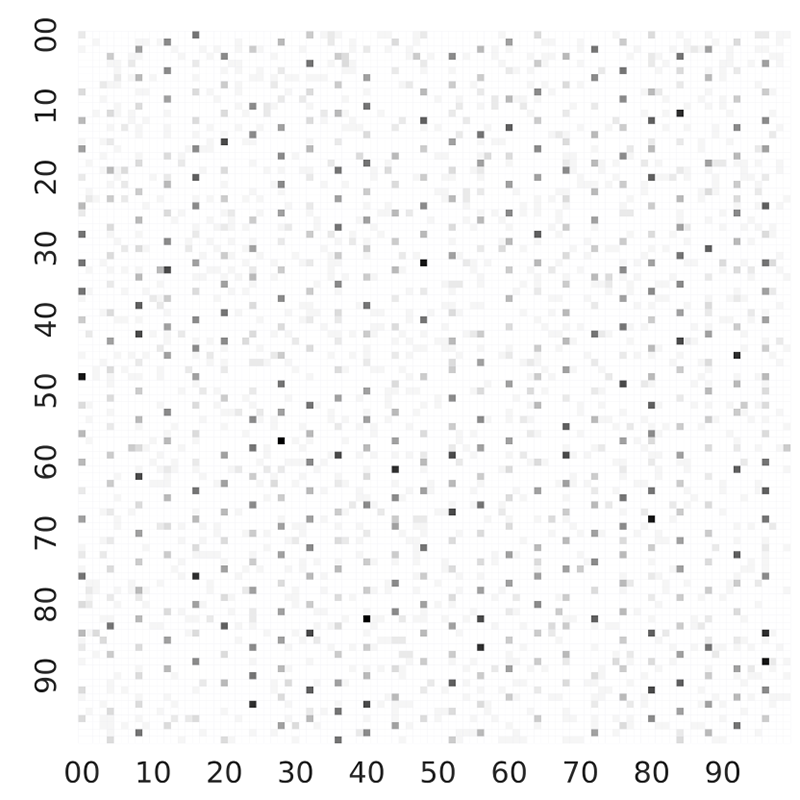
\includegraphics[width=1.1\textwidth]{figures/figure6.png}
                    \caption{WeChat}
                    \label{figure6_WeChat}
                \end{figure}

                \column{.26\textwidth}
                \begin{figure}
                    \centering
                    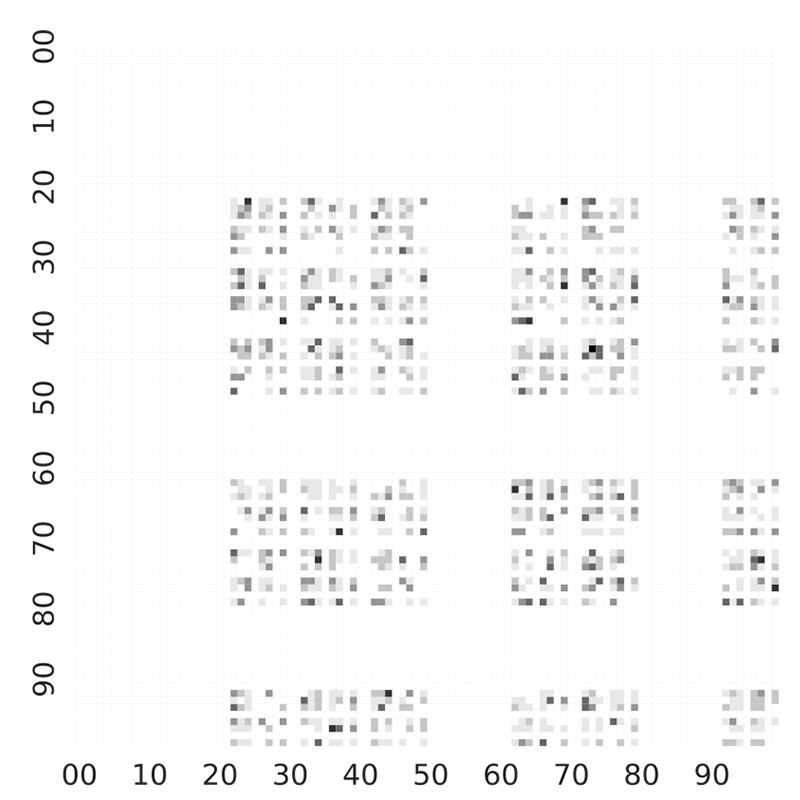
\includegraphics[width=1.1\textwidth]{figures/figure7.png}
                    \caption{Talk2}
                    \label{figure3_Talk2}
                \end{figure}

                \column{.26\textwidth}
                \begin{figure}
                    \centering
                    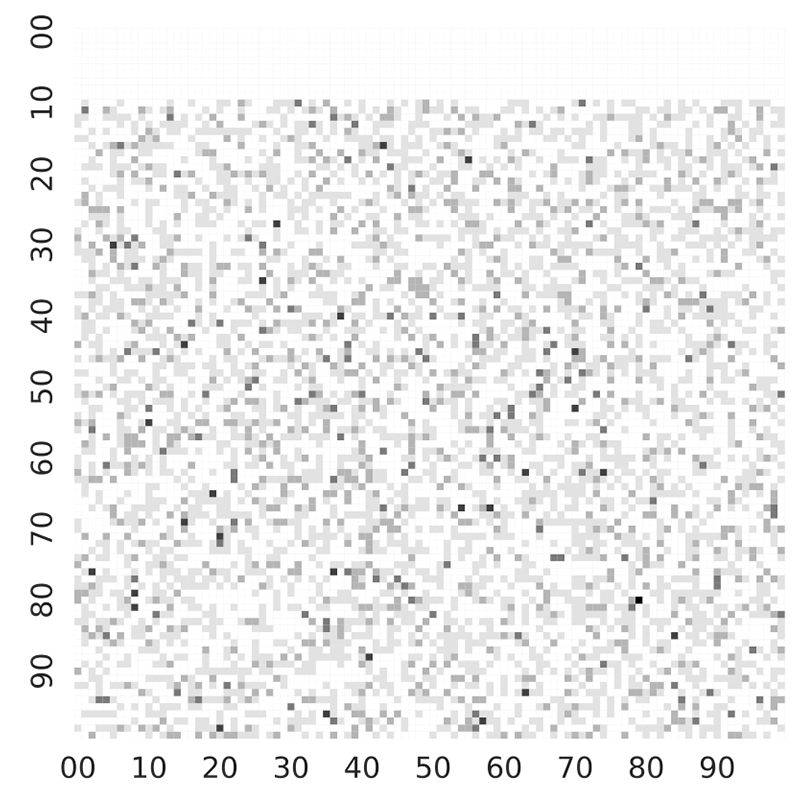
\includegraphics[width=1.1\textwidth]{figures/figure8.png}
                    \caption{Google}
                    \label{figure3_Google}
                \end{figure}

            \end{columns}

		\end{frame}

		\begin{frame}
		  \frametitle{\textbf{SMS的恶意应用}}
            \begin{block}{\textbf{公共网关检测到的恶意信息}}
    		  \begin{itemize}
    		    \item \textbf{泄露用户位置信息}:短URL可以用于确定消息的源和目的地,即会泄漏用户的位置信息。
    		    \item \textbf{垃圾邮件宣传广告}:在公共网关服务中比例较低,约为1.0\%。
                \item \textbf{网络钓鱼活动}:试图欺骗用户,使其相信自己正与合法网站通信。
    		  \end{itemize}
            \end{block}

            \begin{columns}

                \column{.26\textwidth}
                \begin{figure}
                    \centering
                    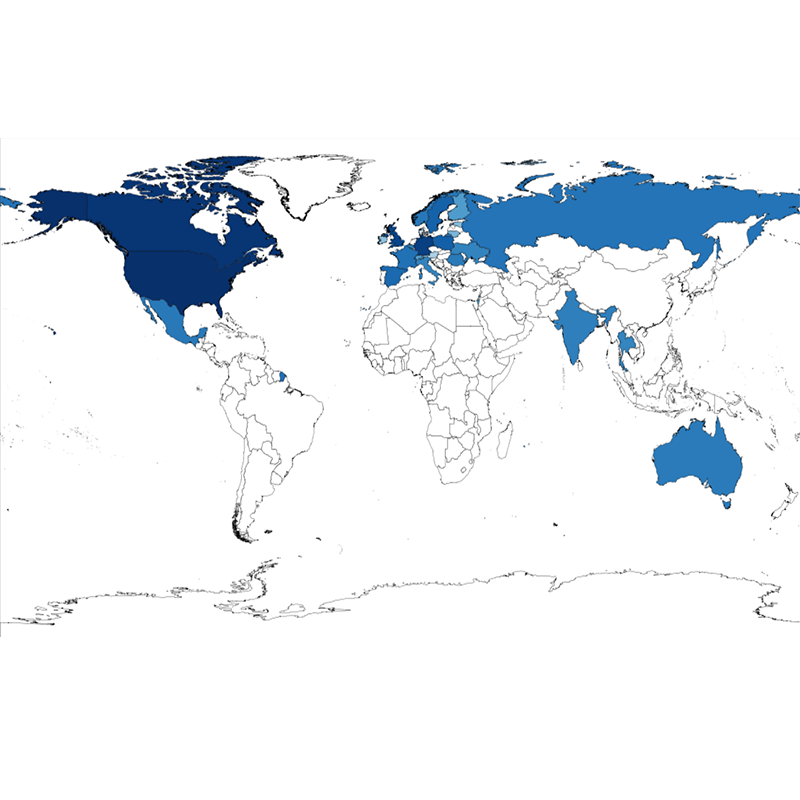
\includegraphics[width=1.1\textwidth]{figures/figure9.png}
                    \caption{SMS地址分布}
                    \label{figure9_WeChat}
                \end{figure}

                \column{.26\textwidth}
                \begin{figure}
                    \centering
                    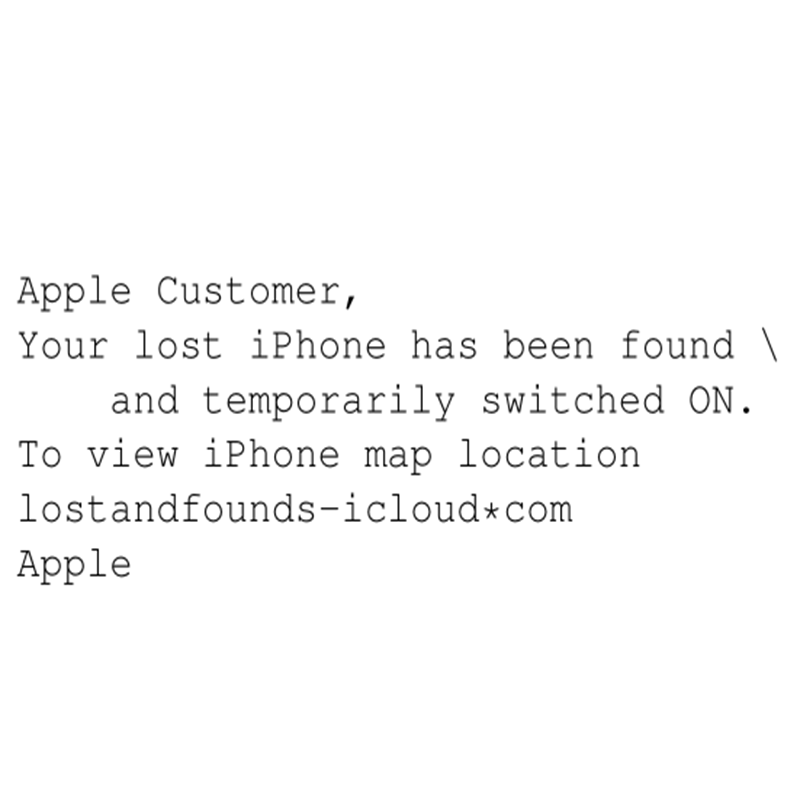
\includegraphics[width=1.1\textwidth]{figures/figure10.png}
                    \caption{钓鱼短信实例}
                    \label{figure10_Talk2}
                \end{figure}

                \column{.26\textwidth}
                \begin{figure}
                    \centering
                    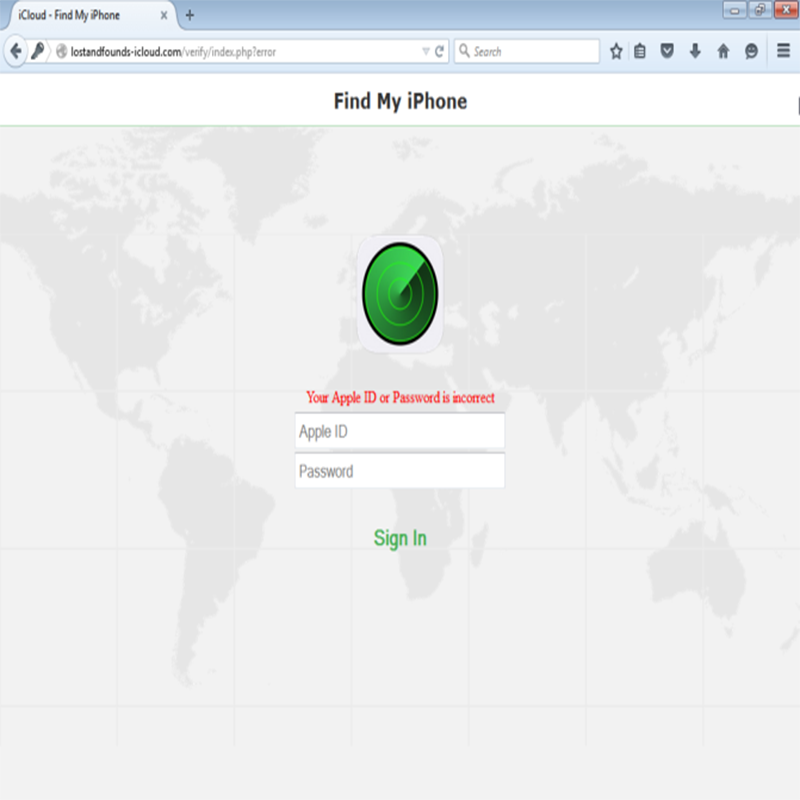
\includegraphics[width=1.1\textwidth]{figures/figure11.png}
                    \caption{钓鱼网站}
                    \label{figure11_Talk2}
                \end{figure}

            \end{columns}

		\end{frame}

\section[结论]{结论}


		\begin{frame}
		  \frametitle{\textbf{结论}}
		
		  \begin{itemize}
		    \item SMS生态系统在智能手机时代出现了新的发展,加入了更多新的设备和参与者。
		    \item 公共网关为用户提供了基于SMS的各种安全解决方案。
            \item 根据该研究,将SMS作为安全信道传递敏感信息存在一定的危险性。一些一次性的消息传递机制亟待改进。
            \item 至于短信滥用,公共网关可以用于规避一些安全性较差的认证机制,或进行PVA欺诈行为。
		  \end{itemize}
		\end{frame}


\section*{}
            \begin{frame}

                \begin{center}
                    \begin{minipage}{1\textwidth}
                        \setbeamercolor{mybox}{fg=white, bg=black!60!green}
                        \begin{beamercolorbox}[wd=0.70\textwidth, rounded=true, shadow=true]{mybox}
                        \LARGE \centering Thanks for Listening.
                        \end{beamercolorbox}
                    \end{minipage}
                \end{center}

                \begin{figure}[!t]
                    \centering
                    
\includegraphics[width=.8\textwidth]{figures/figure5.png}
                    \label{figure4_ad}
                \end{figure}
            \end{frame}

\end{document} 